\documentclass{article}
\usepackage{graphicx}
\usepackage{amsmath}
\usepackage{amsfonts}
\usepackage{amssymb}

\begin{document}

\title{ECE 110 Cramming Carnival Review}
\author{Author: Members of HKN}
\date{Fall 2024}
\maketitle

\section*{Introduction}
This worksheet does not cover content in lectures after November 25th and is not meant to be a replacement for any practice exams or section reviews. Use this worksheet as a quick refresher for various topics throughout the semester and for slightly different questions than the homeworks.

\section*{Formulas not on the help sheet}
\textbf{Note:} All formulas required for the questions are assumed to be known, as they are not provided in this sheet.
\begin{center}
    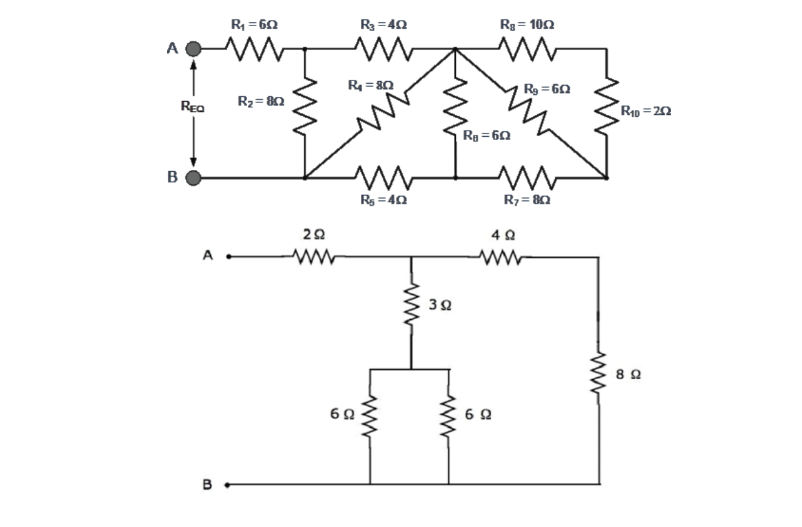
\includegraphics[width=0.75\linewidth]{figures/image.png}
\end{center}
\newpage

\section*{Power Efficiency \& Capacitors}
\textbf{Question 1:} Consider a car that has 400 kJ of energy at a specific speed. The car's regenerative brakes are 40\% efficient at converting kinetic energy to energy stored in a battery. What is the energy added when the car brakes to half speed?

\textbf{Solution:}
% Solution steps
\begin{align*}
    KE_{o} &= \frac{1}{2}mv^{2} \\
    KE_{\text{half}} &= \frac{1}{2} m {\left( \frac{v}{2} \right)}^{2}  = \frac{1}{2} m \cdot \frac{v^{2}}{4}  = \frac{1}{4} \cdot \frac{1}{2} m v^{2} =  \frac{1}{4} \times KE_{o} \\
    \Delta KE &= KE_{o} - KE_{half} = KE_{o} - \frac{1}{4}KE_{o} = \frac{3}{4}KE_{o} \\
    &= \frac{3}{4} \cdot 400kJ = 300 kJ \\
    E_{added} &= \%_{eff} \cdot \Delta KE = 0.40 \cdot 300kJ \\
    &= \boxed{120kJ}
\end{align*}

\textbf{Question 2:} If a 15 kWh battery has to be recharged using a 60\% efficient generator with peak power of 500 W, how long does the generator need to run to fully charge the battery?

\textbf{Question 3:} What is the energy stored in a 4 nF capacitor charged to 9V?

\textbf{Question 4:} What voltage is needed to charge the capacitor from the above question enough to lift a 2-gram mass 15 cm?

\section*{Kirchoff's Laws/Dividers}

\begin{center}
    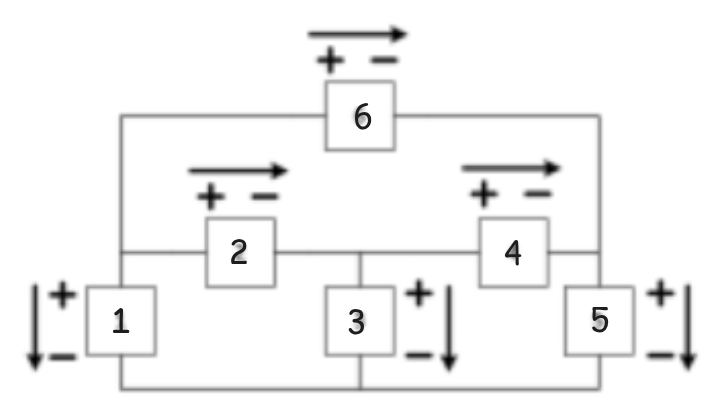
\includegraphics[width=0.75\linewidth]{figures/2.png}
\end{center}

\textbf{Question 5:} Given the above circuit and information, find V1, V3, V6, I2, I4, and I5.

\begin{center}
    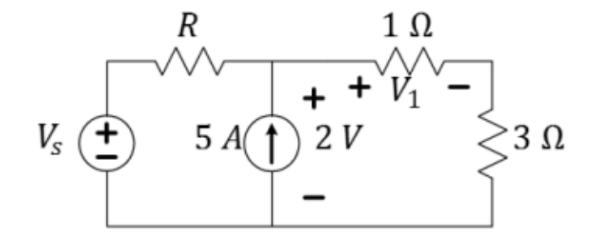
\includegraphics[width=0.75\linewidth]{figures/3.png}
\end{center}

\textbf{Question 6:} Find V1 in the above circuit.

\begin{center}

    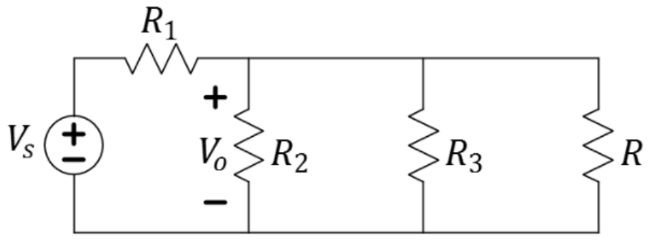
\includegraphics[width=0.75\linewidth]{figures/5.png}

\end{center}


\textbf{Question 7:} What value of R will result in Vo = 1V?

1. We know that the voltage across parallel circuits is the same. As this is the case, if \( V_0 = 1 \, \text{V} \), the voltage at \( R_1 \) is \( 3 \, \text{V} \), since \( V_s = 4 \, \text{V} \).

2. By the voltage divider rule, for \( R_1 \) to be \( 3 \, \text{V} \), the resistance of the three resistors in parallel must be \(\frac{1}{3}\) of that of \( R_1 \). Since \( R_1 = 9 \, \Omega \), the combination of \( R_2, R_3 \), and \( R \) in parallel must be \( 3 \, \Omega \).

3. Thus:
\[
3 = \left( \frac{1}{10} + \frac{1}{15} + \frac{1}{R} \right)^{-1}.
\]

Solving for \( R \), we find:
\[
\frac{1}{R} = \frac{1}{3} - \left( \frac{1}{10} + \frac{1}{15} \right),
\]
\[
\frac{1}{R} = \frac{1}{3} - \frac{1}{6},
\]
\[
\frac{1}{R} = \frac{2}{6} - \frac{1}{6} = \frac{1}{6}.
\]
\[
R = 6 \, \Omega.
\]

\begin{center}
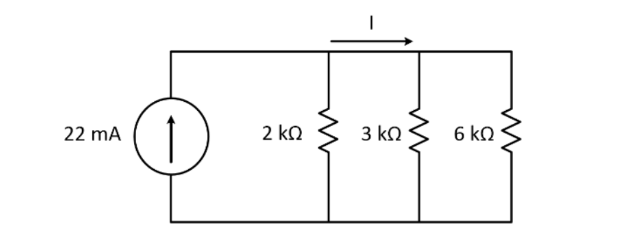
\includegraphics[width=0.75\linewidth]{figures/6.png}
\end{center}

\textbf{Question 8:} Find I in the above circuit.

1. Combine the right two resistors into a single resistor. The resistances are 6 k$\Omega$ and 3 k$\Omega$ in parallel:
\[
R_{\text{eq}} = \left( \frac{1}{6} + \frac{1}{3} \right)^{-1} \text{k}\Omega = \left( \frac{1}{6} + \frac{2}{6} \right)^{-1} \text{k}\Omega = \left( \frac{3}{6} \right)^{-1} \text{k}\Omega = 2 \text{k}\Omega.
\]

2. Use the current divider rule for the two 2 k$\Omega$ resistors in parallel to obtain the current:
\[
I_1 = I_{\text{total}} \cdot \frac{R_2}{R_1 + R_2},
\]
where \( R_1 = R_2 = 2 \text{k}\Omega \).

Substituting values:
\[
I_1 = 22 \text{ mA} \cdot \frac{2}{2 + 2} = 22 \text{ mA} \cdot \frac{1}{2} = 11 \text{ mA}.
\]

\section*{Equivalent Resistance / Power}
\textbf{Question 9:} Find equivalent resistance for the circuits below.

\begin{center}

        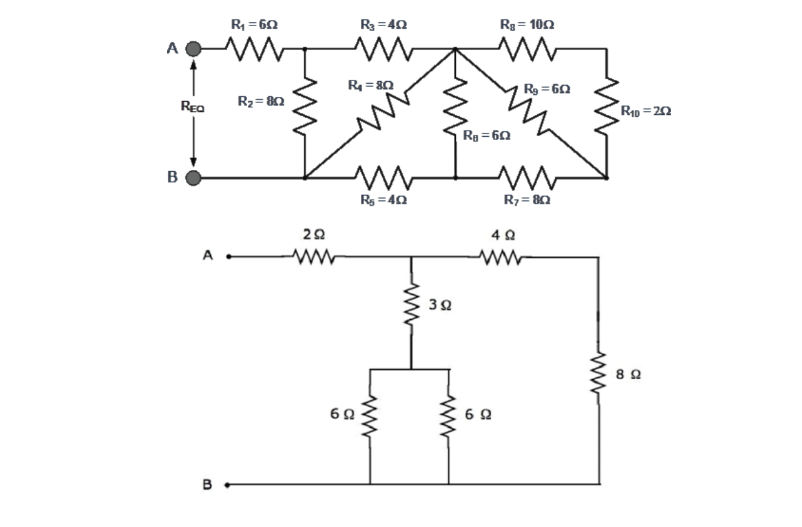
\includegraphics[width=0.75\linewidth]{figures/image.png}
\end{center}

\textbf{Part 1:}

We calculate the equivalent resistance step by step:

1. \( R_8 \) and \( R_{10} \) are in series:  
   \( R_{s1} = R_8 + R_{10} = 12 \, \Omega \).

2. \( R_{s1} \) and \( R_9 \) are in parallel:  
   \( R_{p1} = \left( \frac{1}{R_{s1}} + \frac{1}{R_9} \right)^{-1} = 4 \, \Omega \).

3. \( R_{p1} \) and \( R_7 \) are in series:  
   \( R_{s2} = R_{p1} + R_7 = 12 \, \Omega \).

4. \( R_{s2} \) and \( R_6 \) are in parallel:  
   \( R_{p2} = \left( \frac{1}{R_{s2}} + \frac{1}{R_6} \right)^{-1} = 4 \, \Omega \).

5. \( R_{p2} \) and \( R_5 \) are in series:  
   \( R_{s3} = R_{p2} + R_5 = 8 \, \Omega \).

6. \( R_{s3} \) and \( R_4 \) are in parallel:  
   \( R_{p3} = \left( \frac{1}{R_{s3}} + \frac{1}{R_4} \right)^{-1} = 4 \, \Omega \).

7. \( R_{p3} \) and \( R_3 \) are in series:  
   \( R_{s4} = R_{p3} + R_3 = 8 \, \Omega \).

8. \( R_{s4} \) and \( R_2 \) are in parallel:  
   \( R_{p4} = \left( \frac{1}{R_{s4}} + \frac{1}{R_2} \right)^{-1} = 4 \, \Omega \).

9. \( R_{p4} \) and \( R_1 \) are in series:  
   \( R_{s5} = R_{p4} + R_1 = 10 \, \Omega \).

Thus, the total equivalent resistance is \( R_{\text{eq}} = 10 \, \Omega \).

\bigskip

\textbf{Part 2:}

For the second circuit:

1. The 4$\Omega$ and 8$\Omega$ resistors are in series:  
   \( R_1 = 4 \, \Omega + 8 \, \Omega = 12 \, \Omega \).

2. Two 6$\Omega$ resistors are in parallel:  
   \( R_2 = \left( \frac{1}{6} + \frac{1}{6} \right)^{-1} = 3 \, \Omega \).

3. The 3$\Omega$ from Step 2 and another 3$\Omega$ resistor are in series:  
   \( R_3 = 3 \, \Omega + 3 \, \Omega = 6 \, \Omega \).

4. The 6$\Omega$ from Step 3 and the 12$\Omega$ from Step 1 are in parallel:  
   \( R_4 = \left( \frac{1}{6} + \frac{1}{12} \right)^{-1} = 4 \, \Omega \).

5. The 4$\Omega$ from Step 4 and the 2$\Omega$ resistor are in series:  
   \( R_{\text{eq}} = 4 \, \Omega + 2 \, \Omega = 6 \, \Omega \).

Thus, the total equivalent resistance is \( R_{\text{eq}} = 6 \, \Omega \).
\bigskip


\textbf{Question 10:} If the voltage between nodes A and B in the second circuit is 9V...
\begin{enumerate}
\item What is the current through the 3 ohm resistor?
\\
\\
We know from Question 9 that the equivalent resistance \( R_{\text{eq}} = 6 \, \Omega \). Using Ohm's law, the total current flowing through the circuit is:
    \[
    I_{\text{total}} = \frac{V}{R_{\text{eq}}} = \frac{9V}{6 \, \Omega} = 1.5 \, \text{A}.
    \]
    Using the current divider rule, we can find the current through the middle branch, which has a resistance of 6\(\Omega\) (the combination of 3\(\Omega\) and two 6\(\Omega\) resistors in parallel):
    \[
    R_{\text{middle}} = 3 \, \Omega + \left( \frac{1}{6} + \frac{1}{6} \right)^{-1} = 3 \, \Omega + 3 \, \Omega = 6 \, \Omega.
    \]
    The current divides between the middle branch and the right branch with resistance 12\(\Omega\) (the 4\(\Omega\) and 8\(\Omega\) resistors in series). By the current divider rule:
    \[
    I_{\text{middle}} = I_{\text{total}} \times \frac{R_{\text{right}}}{R_{\text{middle}} + R_{\text{right}}} = 1.5 \, \text{A} \times \frac{12 \, \Omega}{6 \, \Omega + 12 \, \Omega} = 1 \, \text{A}.
    \]
    Thus, the current through the 3\(\Omega\) resistor is \( 1 \, \text{A} \).
\\
\item What is the power through the 3 ohm resistor?
\\
\\
The power dissipated through a resistor is given by \( P = I^2 R \). For the 3\(\Omega\) resistor:
    \[
    P_3 = I_{\text{3}\Omega}^2 \times 3 \, \Omega = (1 \, \text{A})^2 \times 3 \, \Omega = 3 \, \text{W}.
    \]


\item What is the power through the 8 ohm resistor?
\\
\\
The current through the 8\(\Omega\) resistor is the same as the current through the right branch, which is:
    \[
    I_{\text{8}\Omega} = I_{\text{total}} - I_{\text{middle}} = 1.5 \, \text{A} - 1 \, \text{A} = 0.5 \, \text{A}.
    \]
    The power dissipated through the 8\(\Omega\) resistor is:
    \[
    P_8 = I_{\text{8}\Omega}^2 \times 8 \, \Omega = (0.5 \, \text{A})^2 \times 8 \, \Omega = 2 \, \text{W}.
    \]

\item What resistor has the highest power output?
\\
\\
Since power is given by \( P = I^2 R \), we can analyze the power dissipated in each resistor.

- The 4\(\Omega\) resistor and the 8\(\Omega\) resistor have the same current flowing through them. Since the current is the same, we know the 4\(\Omega\) resistor does not have the highest power output. 
\\
- The 3\(\Omega\) resistor dissipates more power than the 8\(\Omega\) resistor, as we computed earlier, and the power dissipated in each of the 6\(\Omega\) resistors in parallel is \( P = 0.5^2 \times 6 = \frac{3}{2} \, \text{W} \).
\\
- The power through the 2\(\Omega\) resistor is \( P = 1.5^2 \times 2 = 4.5 \, \text{W} \).

Thus, the 2\(\Omega\) resistor has the highest power output.
\end{enumerate}

\section*{PWM}
\textbf{Question 11:} Imagine a square wave that outputs 15W from 0 to 12 seconds and 5W from 12 to 20 seconds. This square wave corresponds to a 10 ohm resistor.
\begin{enumerate}
    \item What is the Average Power of this waveform?
    \item What is the RMS Voltage of this waveform?
\end{enumerate}
\textbf{Question 12:} Given a limited portion of this graphed waveform, what is its duty cycle?

\begin{center}

        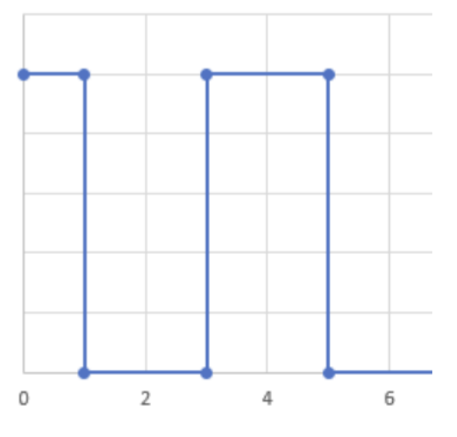
\includegraphics[width=0.75\linewidth]{figures/8.png}
\end{center}

\pagebreak

\section*{I-V Equations}
\textbf{Question 13:} What is the short circuit current and the open circuit voltage for the circuit below?
\begin{center}

        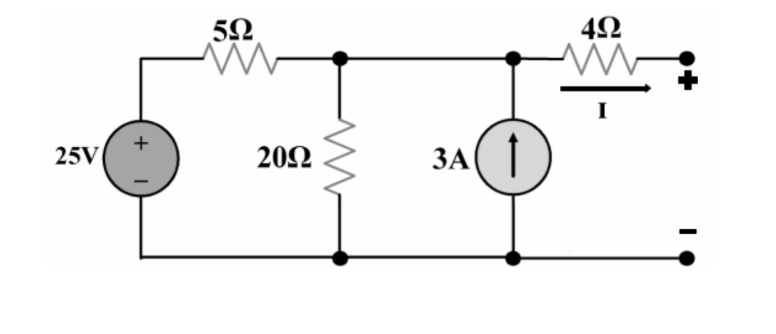
\includegraphics[width=0.75\linewidth]{figures/12.png}

\end{center}

\textbf{Question 14:} If this circuit were to be placed in series with another circuit with an IV equation of \(I = 0.005V - 0.025\), assuming the same polarities given above, what would be the operating current and voltage?

\textbf{Question 15:} If the open circuit voltage of a circuit containing ideal sources and resistors is measured at Voc = 8 V, while the current through the short circuit across the circuit is Isc = 200 mA, what would be the power in watts absorbed by an ideal voltage source, Vs = 4, placed across the terminals?

\begin{center}
    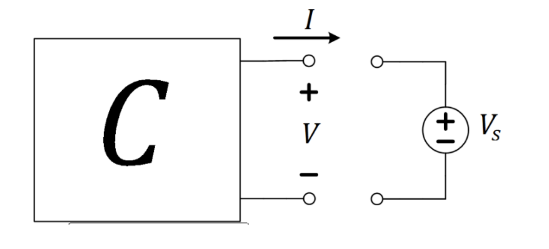
\includegraphics[width=0.75\linewidth]{figures/14.png}

\end{center}

\section*{Norton and Thevenin}
\textbf{Question 16:} Give Norton and Thevenin Forms for the subcircuit shown on the previous page.

\textbf{Question 17:} What is the Norton resistance of the circuit below? What is the Thevenin Resistance?

\textbf{Question 18:} Draw the Thevenin and Norton Equivalents.

\begin{center}
    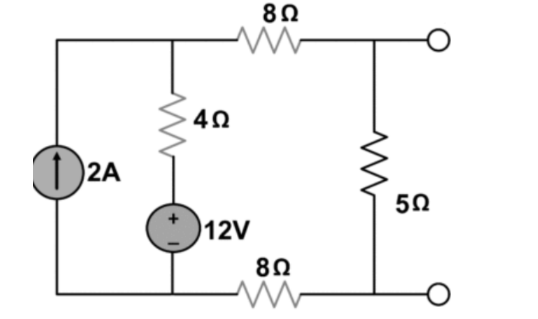
\includegraphics[width=0.75\linewidth]{figures/23.png}

\end{center}

\section*{Nodal Analysis}
\textbf{Question 19:} Find the voltage at node A for this circuit.

\textbf{Question 20:} Find the voltage drop across the 10, 30, and 50 ohm resistors.

\begin{center}
    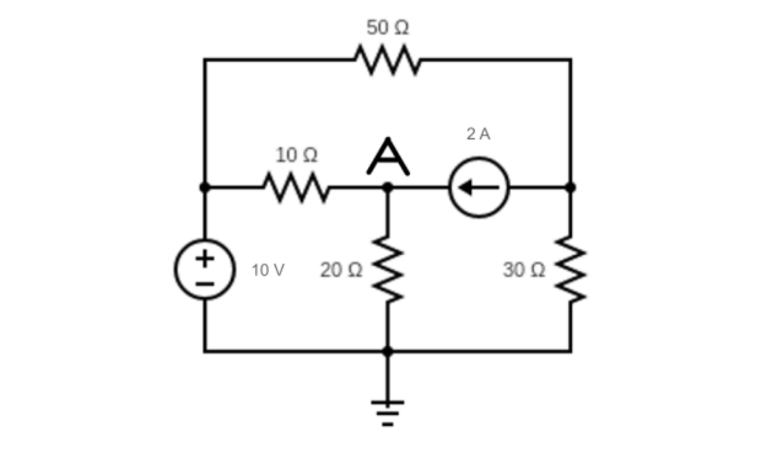
\includegraphics[width=0.75\linewidth]{figures/34.png}
\end{center}

\pagebreak

\section*{Diodes}
\textbf{Question 21:} Assume an ideal-offset model and Von = 1 volt. If Vs = 5 cos(\(\omega\)t) volts and V1 = 2 volts, what are the maximum and minimum voltages across the open nodes?

\begin{center}

        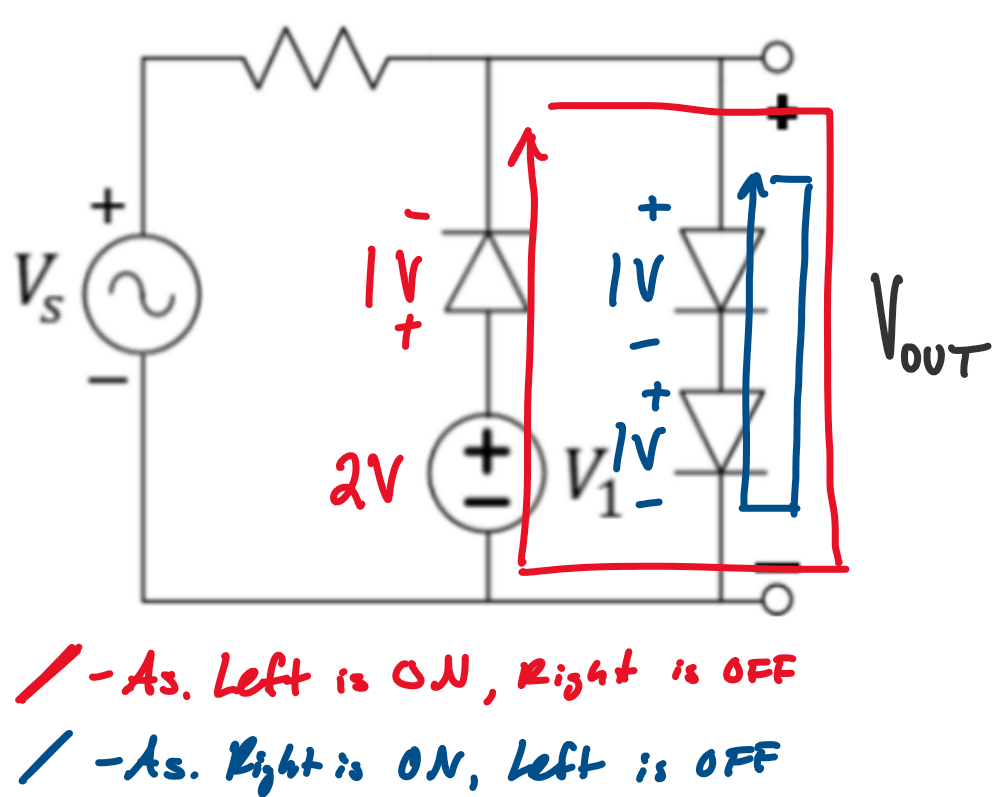
\includegraphics[width=0.75\linewidth]{figures/21_sol.png}
\end{center}

\textbf{Solution:} 
Both branches of the diode cannot be ON at the same time, as if positive current flows through one, negative current would flow through the other (which is impossible). We start by solving for $V_{out}$ assuming one diode configuration is ON (below, we start with the left branch) while the other is OFF.

KVL Loops are shown above with assumptions the Voltage source has extremes high or low enough that they will conduct current.
\begin{align*}
    V_{out} = 2V-1V = 1V.
\end{align*}
\indent For current to flow in the correct direction, the voltage on the right of the resistor must have a larger value than the voltage on the left. We have determined $V_{out} = 1V$, we now check whether $V_S$ can be smaller than that number.
\begin{align*}
    V_{S\min} = -5V < 1V \Rightarrow \boxed{V_{out\min} = 1V}
\end{align*}
\indent Restart this process with the KVL loop with the right branch of diodes. 
\begin{align*}
    V_{out} = 1V+1V = 2V
\end{align*}
\indent Current must flow in the resistor from left to right to satisfy the diode assumption. Find a value of $V_S$ that is greater than our calculated $V_{out}$
\begin{align*}
    V_{S\max} = 5 > 2V \Rightarrow \boxed{V_{out\max} = 2V}
\end{align*}


\textbf{Question 22:} In the circuit below, which diodes are on? Furthermore, if Vs = 10 V, all the diodes have Von = 2V under the offset ideal model, and the voltage drop over R1 is also 2V, what is the voltage drop across the other resistors, assuming they have an equal resistance?

\begin{center}
    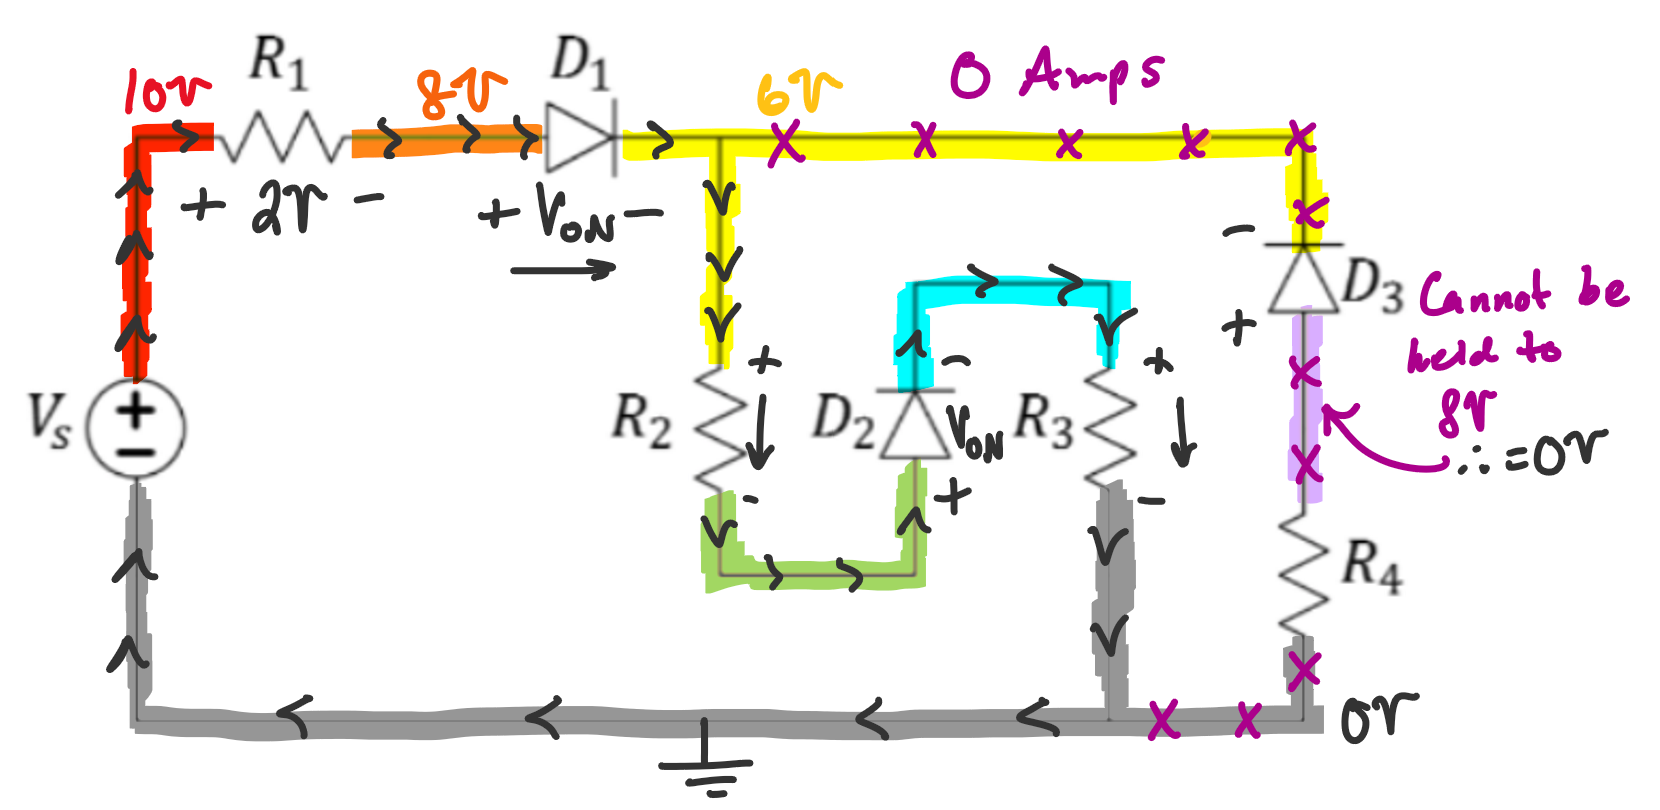
\includegraphics[width=0.75\linewidth]{figures/q22_sol.png}
\end{center}

\textbf{Solution:} 

When looking at $D_3$, we notice two things:
\begin{itemize}
    \item The \textbf{positive} terminal of $D_3$ is connected to the \textbf{negative} terminal of $V_S$ through a resistor.
    \item There is only one source of power in the circuit ($V_S$). (Because of this, the smallest nodal voltage that any node could be held at is 0V (the negative terminal of the $V_S$))
\end{itemize}

Thus, it is impossible for the voltage difference across the diode, $V_{D_3}$, to be greater than $0V$. In fact, if we assume $D_1$ to be on, we can calculate that $V_{yellow} = V_S - V_{R_1} - V_{ON} = 6V$. $V_{pink}$ would need to be $2V$ greater than $V_{yellow}$ in order for $D_3$ to turn on. Since a resistor is a passive component (adds no power to the circuit), it is impossible to raise the pink node to above $6V+2V = 8V$, which would allow $D_3$ to turn on 

Since $D_3$ is not conducting any current, $I_{R_1} = I_{R_2} = I_{R_3} = I_{D_1} = I_{D_2} > 0A $. 
We know the currents will be positive since $R_1$'s voltage drop is positive and moving away from the voltage source 
(no other supply of power in the circuit). 
Because the currents are all positive, we can conlcude that \boxed{D_1 \text{ and } D2 \text{ are ON}}. 
For any two resistors of equal resistance and equal current, 
we know that their voltage drops must also be equal.
 Algebraically, we can show this as follows:
\begin{align*}
    I_{R_1} &= I_{R_2} = I_{R_3} \\
    \text{Using Ohm's Law: }\frac{2V}{R} &= \frac{V_{R_2}}{R} = \frac{V_{R_3}}{R} \\
    2V &= V_{R_2} = V_{R_3} \\ 
    V_{R_2} &= \boxed {2V } \\
    V_{R_3} &= \boxed {2V }
\end{align*} 



\pagebreak

\section*{BJTs}
\textbf{Question 23:} The properties of the transistor are that VBE on is 1V, \(\beta\) is 120, and VCE sat is 0.2 V. In this circuit, VCC is 9V, RC is 150\(\Omega\), and RB is 30000\(\Omega\). What are the maximum and minimum values for VCE if Vi’s output is variable between 0V and 9V?

\begin{center}

    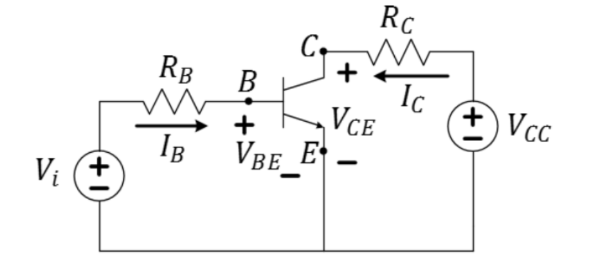
\includegraphics[width=0.75\linewidth]{figures/56.png}
\end{center}

\textbf{Solution:} 

An important property of BJTs is that $V_{CE}$ can only ever assume the values ranging from $[V_{CE,sat},V_{CC}]$. A great graph to view that displays the behavior of a BJT is Figure 6 of the Canvas Module, "BJT Applications."

Calculate $V_{CE}$ assuming that the BJT is in the ON, ACTIVE region for both extreme values of $V_i$:
\begin{itemize}
    \item If $I_C \le 0$ (equivalent statements: $V_{CE} > V_{CC}$, $V_i < V_{BE,ON}$), then the assumption that the BJT is ON is incorrect, and $V_{CE}$'s actual value is $V_{CC}$.
    \item If $V_{CE,sat} < V_{CE} < V_{CC}$, then the assumption that the BJT is in the ON, ACTIVE region is correct and the calculated value of $V_{CE}$ is correct.
    \item If $V_{CE} \le V_{CE,sat}$, then the BJT is in the ON, SATURATED region and $V_{CE}$'s actual value is $V_{CE,sat}$.
\end{itemize}

We see that $V_I$ gets below the value of $V_{BE,ON}$, so we know that
\begin{center}
    \boxed{V_{CE,max} = V_{CC} = 9V}.
\end{center}

Assuming the BJT is in the active region: 
\begin{align*}
    I_C &= \beta I_B \\
    \frac{V_{CC}-V_{CE,min}}{R_C} &= \beta \frac{V_{i,max} - V_{BE,on}}{R_B} \\
    \Rightarrow V_{CE,min} &= V_{CC} - \beta\frac{R_C(V_{i,max} - V_{BE,on})}{R_B} \\
    V_{CE,min} &= 9V - (120)\frac{(150\Omega)(9V-1V)}{30k\Omega} \\
    V_{CE,min}&= \boxed{4.2V} \text{ (within bounds } V_{CE,sat}<V_{CE}< V_{CC}. \text{)}
\end{align*} 

\vspace{5mm}

\textbf{Question 24:} If Vi was set to 5V, what would VCE be?

\textbf{Solution:}

Assume that the BJT is in the active region: 
\begin{align*}
    I_C &= \beta I_B \\
    \frac{V_{CC}-V_{CE}}{R_C} &= \beta \frac{V_i - V_{BE,on}}{R_B} \\
    \Rightarrow V_{CE} &= V_{CC} - \beta\frac{R_C(V_i - V_{BE,on})}{R_B} \\
    V_{CE} &= 9V - (120)\frac{(150\Omega)(5V-1V)}{30k\Omega} \\
    &= \boxed{6.6V} \text{ (within bounds } V_{CE,sat}<V_{CE}< V_{CC}. \text{)}
\end{align*}

Since $V_{CE}$ is in the range $V_{CE,sat} < V_{CE} < V_{CC}$, we know our assumption that the BJT was in the active region is correct, and our calculated $V_{CE}$ is correct.


\section*{MOSFETs/cMOS logic}
\textbf{Question 25:} An IC dissipates 110W. If the IC has a 5\% activity factor \(\alpha\), frequency of 10GHz, and 1nF gate capacitance, what is the maximum number of transistors that can be in the IC if it can operate at up to 9V?

\begin{center}

        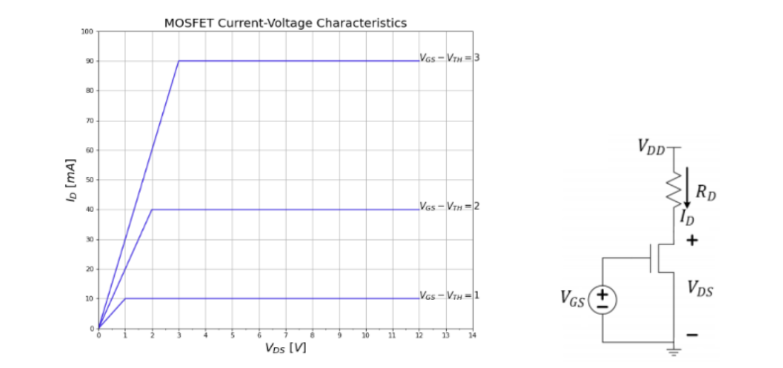
\includegraphics[width=1\linewidth]{figures/78.png}
\end{center}

\textbf{Question 26:} The given circuit with a MOSFET in series with a voltage source of 6V and a resistor with a resistance of 120\(\Omega\)
Find the transistor parameter k and a value for VDS that results in I = 30 mA, given that VGS - VTH = 2.

\section*{Bonus Questions}

\textbf{Question 27:} Give the IV equation, Norton equivalent, and Thevenin Equivalent for the circuit below.

\begin{center}

    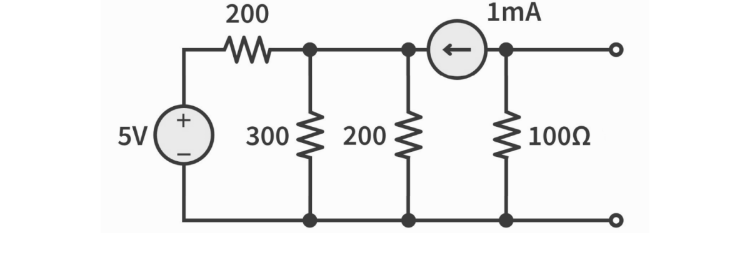
\includegraphics[width=0.75\linewidth]{figures/99.png}
\end{center}

\end{document}